% PointWorld presenter deck. CS 2883R, 18 Nov 2026. Juntang Wang, Vivian Hui.
% Numbers from arXiv 2601.03782v1; frame comments name the source. l2 is in metres.
% Presenter speaks as first author; critique lives in Discussion and "Backup: our reading".
% 15:00: Vivian S1-3 (~8:00), Juntang S4-6 (~7:00). If long, trim Data and Real robot.
% LAPA deck: tag lapa-final. Build: latexmk -pdf main.tex
\documentclass[aspectratio=169,12pt]{beamer}
\usetheme[progressbar=none, numbering=counter]{moloch}
\usepackage[sfdefault,light]{FiraSans}
\usepackage[T1]{fontenc}
\usepackage{tikz}
\usepackage{booktabs}
\usepackage{multicol}
\usepackage[authoryear, round]{natbib}
\definecolor{cite}{HTML}{1F5FBF}  % citations and URLs: blue, clickable
\hypersetup{colorlinks=true, citecolor=cite, urlcolor=cite, linkcolor=.}
\renewcommand{\bibsection}{}                          % the frame title is enough
\bibliographystyle{plainnat}
% natbib fix: Beamer + hyperref drop the ", " in author-year citations.
\makeatletter
\AddToHook{begindocument/end}{%
  \def\hyper@natlinkbreak#1#2{\hyper@linkend#1\hyper@linkstart{cite}{cite.#2}}}
\makeatother

\definecolor{ink}{HTML}{222222}
\definecolor{mute}{HTML}{8a8a8a}
\definecolor{pw}{HTML}{12807A}       % PointWorld rows and accents
\definecolor{crimson}{HTML}{A51C30}  % Harvard; title slide only

\setbeamercolor{normal text}{fg=ink, bg=white}
\setbeamercolor{frametitle}{fg=ink, bg=white}
\setbeamercolor{page number in head/foot}{fg=mute}
\setbeamertemplate{itemize items}{\color{pw}--}
\setlength{\leftmargini}{1.1em}

\newcommand{\src}[1]{{\scriptsize\color{mute}\citep{#1}}}
\newcommand{\paperfig}[3]{%
  \begin{tikzpicture}[baseline=(f.south)]
    \node[inner sep=0pt] (f) {\includegraphics[#1]{#2}};
    \node[anchor=north east, inner sep=1pt, font=\tiny, text=mute] at (f.south east)
      {\citet{huang2026pointworld}, #3};
  \end{tikzpicture}}
\newcommand{\credit}[1]{\par\hfill{\tiny\color{mute}\citet{huang2026pointworld}, #1}\par}
\newcommand{\pw}[1]{{\color{pw}#1}}
\newcommand{\colhead}[2]{\begin{minipage}[t][1.5cm]{\linewidth}\raggedright
  {\small\bfseries #1}\\\src{#2}\end{minipage}\\}
\newenvironment{notes}[1][\linewidth]
  {\begin{minipage}{#1}\footnotesize\begin{itemize}\setlength{\itemsep}{2pt}}
  {\end{itemize}\end{minipage}}

\begin{document}

% Title
\begin{frame}[plain]
  \vfill
  {\LARGE\bfseries PointWorld: Scaling 3D World Models\\[2pt]
    for In-The-Wild Robotic Manipulation}\\[6pt]

  {\scriptsize\color{mute} Wenlong Huang, Yu-Wei Chao, Arsalan Mousavian, Ming-Yu Liu,
    Dieter Fox, Kaichun Mo, Li Fei-Fei.\\ Stanford, NVIDIA.\
    CVPR 2026. arXiv 2601.03782. Code, data and checkpoints: github.com/NVlabs/PointWorld}

      \textcolor{crimson}{\rule{\textwidth}{0.8pt}}\\[8pt]
  Juntang Wang $\cdot$ Vivian Hui\\[2pt]
  \vfill
\end{frame}



\begin{frame}{What is PointWorld?}
  \vfill
  \centering
  \begin{minipage}{0.92\textwidth}
    \large\raggedright
    ``POINTWORLD, a \textbf{large pre-trained 3D world model} that
    unifies \textbf{state and action} in a \textbf{shared 3D space}
    as \textbf{3D point flows}: given one or few RGB-D images and
    a sequence of low-level robot action commands, POINTWORLD
    forecasts \textbf{per-pixel displacements in 3D} that respond
    to the given actions.''
  \end{minipage}
  \vfill
  \credit{Abstract; emphasis added}
\end{frame}

%% ---- Part A (Vivian, S1-3) ----
\newcommand{\lossmark}[3]{\ifnum#1=#2\relax{\color{orange!90!red}\setlength{\fboxrule}{2pt}\setlength{\fboxsep}{2.5pt}\boxed{\color{ink}#3}}\else#3\fi}
\newcommand{\pwequation}[1]{%
\[
\mathcal L=\tfrac12\sum_{k,i}^{H,N_S}
\lossmark{#1}{2}{w_{k,i}}
\Big(
\lossmark{#1}{1}{\rho_\delta(\hat{\mathbf P}_{t+k,i}-\mathbf P_{t+k,i})}
\lossmark{#1}{3}{e^{-s_{k,i}}}
+\lossmark{#1}{4}{s_{k,i}}
\Big).
\]}
\begin{frame}{Context: why do robots need world models?}
  \centering
  \paperfig{height=3.55cm}{figs/fig1_teaser.pdf}{Fig.~1}
  \vfill
  \begin{notes}[0.92\linewidth]
    \item<1-> A robot must anticipate how an action changes its surroundings before committing to it.
    \item<2-> A \textbf{world model} predicts future scene states from the current observation and a proposed action.
    \item<3-> \pw{Use these predictions to compare actions and plan physical interactions in unseen environments.}
  \end{notes}
  \vfill
\end{frame}

\newcommand{\approachcrop}[6]{%
  \begin{tikzpicture}
    \node[anchor=south west,inner sep=0pt] (ref) at (0,0)
      {\phantom{\includegraphics[width=#1]{#2}}};
    \begin{scope}[x={(ref.south east)},y={(ref.north west)}]
      \clip (#3,#4) rectangle (#5,#6);
      \node[anchor=south west,inner sep=0pt] at (0,0)
        {\includegraphics[width=#1]{#2}};
    \end{scope}
    \pgfresetboundingbox
    \begin{scope}[x={(ref.south east)},y={(ref.north west)}]
      \path[use as bounding box] (#3,#4) rectangle (#5,#6);
    \end{scope}
  \end{tikzpicture}%
}

\begin{frame}[t]{Related work: approaches to predicting physical interactions}
\vspace{-0.9cm}

\begin{columns}[t]

% ----- Physics simulators -----
\column{0.31\textwidth}
\uncover<1->{
  \begin{minipage}[t][0.8cm]{\linewidth}
    {\small\bfseries Physics simulators}\par
  \end{minipage}\par

  \begin{minipage}[c][1.95cm][c]{\linewidth}
    \centering
    \resizebox{!}{1.9cm}{%
      \approachcrop{8cm}{approach_mujoco.png}
        {0.30}{0.16}{0.72}{0.85}}
  \end{minipage}\par

  {\tiny\color{mute}
    \href{https://mujoco.readthedocs.io/en/stable/models.html}
      {MuJoCo Menagerie: Franka Panda}}\par

  \vspace{2pt}
  {\scriptsize
    \begin{itemize}
      \setlength{\itemsep}{3pt}
      \setlength{\parskip}{0pt}
      \setlength{\topsep}{2pt}
      \item Simulate physical interactions using equations,
        scene geometry, and specified physical properties.
      \item Require scene-specific setup, and simulated
        behavior can differ from reality.
    \end{itemize}
  }
}

% ----- Video generative models -----
\column{0.31\textwidth}
\uncover<2->{
  \begin{minipage}[t][0.8cm]{\linewidth}
    {\small\bfseries Video generative models}\par
  \end{minipage}\par

  \begin{minipage}[c][1.95cm][c]{\linewidth}
    \centering
    \resizebox{!}{1.9cm}{%
      \approachcrop{8cm}{approach_cosmos.jpg}
        {0.56}{0.25}{0.94}{0.82}}
  \end{minipage}\par

  {\tiny\color{mute}
    \href{https://www.nvidia.com/en-us/ai/cosmos/}
      {NVIDIA Cosmos: video generation}}\par

  \vspace{2pt}
  {\scriptsize
    \begin{itemize}
      \setlength{\itemsep}{3pt}
      \setlength{\parskip}{0pt}
      \setlength{\topsep}{2pt}
      \item Learn from video data to generate videos
        conditioned on inputs such as text or images.
      \item Realistic appearance does not guarantee accurate
        physics or precise robot-action control.
    \end{itemize}
  }
}

% ----- Learned dynamics models -----
\column{0.31\textwidth}
\uncover<3->{
  \begin{minipage}[t][0.8cm]{\linewidth}
    {\small\bfseries Learned dynamics\\models}\par
  \end{minipage}\par

  \begin{minipage}[c][1.95cm][c]{\linewidth}
    \centering
    \resizebox{!}{1.9cm}{%
      \approachcrop{8cm}{approach_dreamer.png}
        {0}{0.15}{0.51}{1}}
  \end{minipage}\par

  {\tiny\color{mute}
    \href{https://github.com/danijar/dreamerv3}
      {DreamerV3 (Hafner et al., 2025)}}\par

  \vspace{2pt}
  {\scriptsize
    \begin{itemize}
      \setlength{\itemsep}{3pt}
      \setlength{\parskip}{0pt}
      \setlength{\topsep}{2pt}
      \item Learn from interaction data to predict how
        the environment changes in response to actions.
      \item \textbf{Example: Dreamer} encodes a game screen
        into a latent state, then predicts how it changes
        after an action such as ``move right.''
    \end{itemize}
  }
}

\end{columns}
\vfill
\end{frame}

% Crops from the same example in Figure 2.
\newcommand{\pwvisualcrop}[5]{%
  \begin{tikzpicture}
    \node[anchor=south west,inner sep=0pt] (ref) at (0,0)
      {\phantom{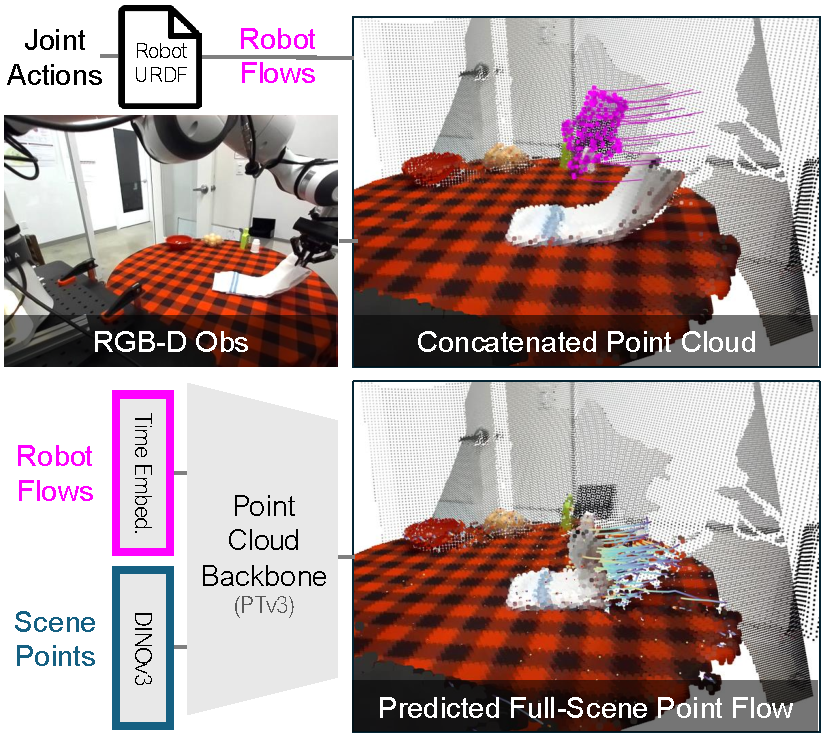
\includegraphics[width=#1]{figs/fig2_overview.pdf}}};

    \begin{scope}[x={(ref.south east)},y={(ref.north west)}]
      \clip (#2,#3) rectangle (#4,#5);
      \node[anchor=south west,inner sep=0pt] at (0,0)
        {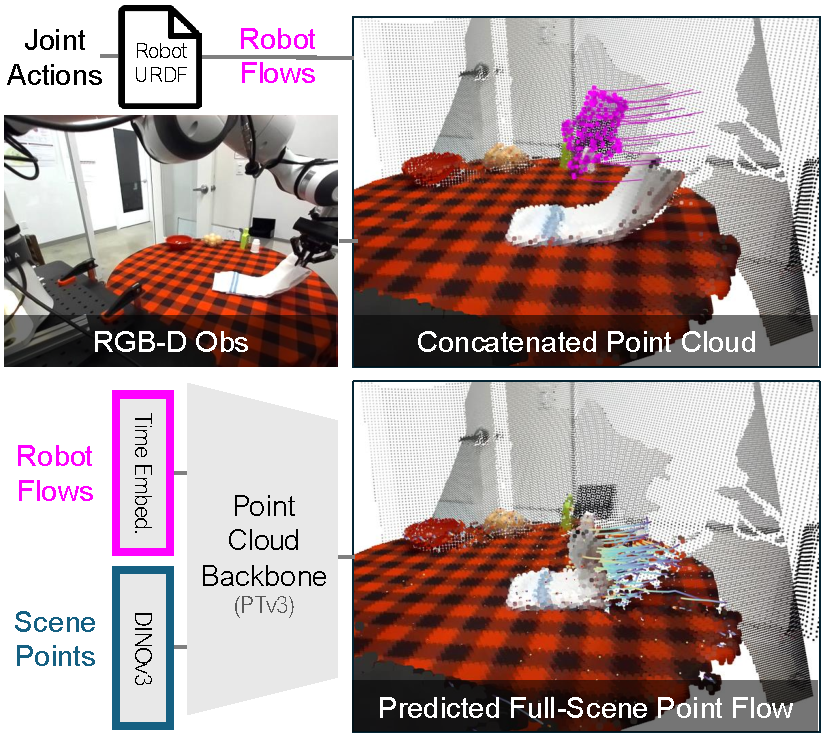
\includegraphics[width=#1]{figs/fig2_overview.pdf}};
    \end{scope}

    \pgfresetboundingbox
    \begin{scope}[x={(ref.south east)},y={(ref.north west)}]
      \path[use as bounding box]
        (#2,#3) rectangle (#4,#5);
    \end{scope}
  \end{tikzpicture}%
}

\begin{frame}[t]{Motivation: why use 3D point flows?}
  \vspace{-0.2cm}
  \footnotesize
  \begin{itemize}\setlength{\itemsep}{12pt}
    \item<1-> \textbf{\color{pw}Geometry for physical interaction}\\
      3D positions directly describe distances and contact geometry,
      rather than visual appearance alone.

    \item<2-> \textbf{\color{pw}A common format across robots}\\
      Point trajectories can describe different gripper shapes and
      robot embodiments without a fixed, robot-specific action vector.

    \item<3-> \textbf{\color{pw}Direct motion supervision}\\
      Corresponding scene points provide displacement targets.

    \item<4-> \textbf{\color{pw}Fewer required annotations}\\
      No explicit object segmentation or material labels are required
      as model inputs.
  \end{itemize}
  \vfill
  \credit{\S1--3.1}
\end{frame}

\begin{frame}[t]{PointWorld: state and action share 3D space}
\vspace{-0.35cm}
\centering

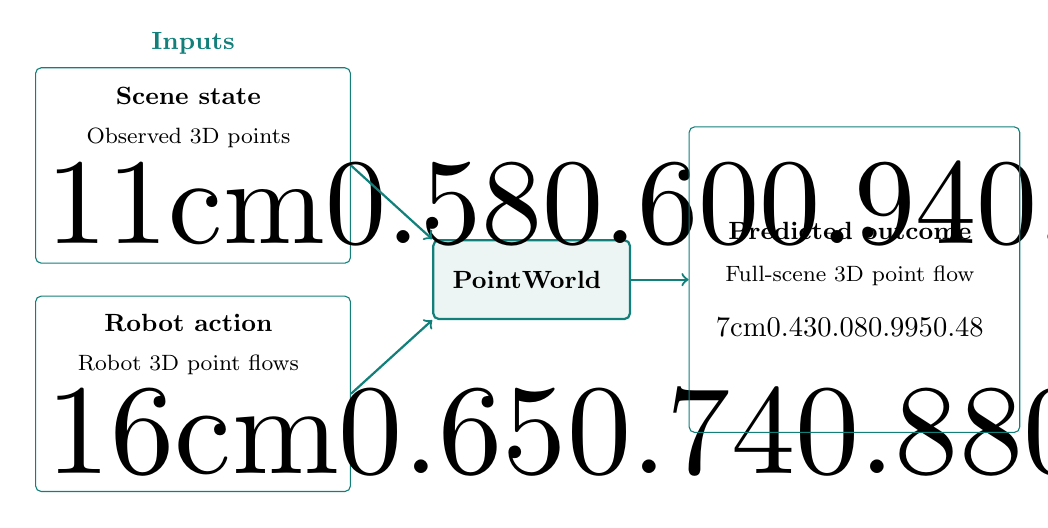
\begin{tikzpicture}[
  panel/.style={
    draw=pw,
    rounded corners=2pt,
    inner sep=4pt,
    align=center
  },
  model/.style={
    draw=pw,
    thick,
    fill=pw!8,
    rounded corners=2pt,
    minimum height=1cm,
    inner sep=7pt,
    align=center
  }
]

% Fixed bounds prevent movement between reveals.
\path[use as bounding box]
  (-2.1,-2.8) rectangle (10.5,3.2);

\node[font=\small\bfseries,text=pw]
  at (0,3.0) {Inputs};

% PointWorld model.
\node[model] (pwmodel) at (4.3,0) {
  \mbox{\small\bfseries PointWorld}
};

% Input 1: observed scene state.
\uncover<1->{
  \node[panel] (scene) at (0,1.45) {
    \begin{minipage}[c][2.2cm][c]{3.6cm}
      \centering

      {\small\bfseries Scene state}\par
      \vspace{2pt}

      {\footnotesize Observed 3D points}\par
      \vspace{5pt}

      \resizebox{!}{1cm}{%
        \pwvisualcrop{11cm}{0.58}{0.60}{0.94}{0.76}}
    \end{minipage}
  };

  \draw[->,thick,pw]
    (scene.east) -- (pwmodel.north west);
}

% Input 2: proposed robot action.
\uncover<2->{
  \node[panel] (action) at (0,-1.45) {
    \begin{minipage}[c][2.2cm][c]{3.6cm}
      \centering

      {\small\bfseries Robot action}\par
      \vspace{2pt}

      {\footnotesize Robot 3D point flows}\par
      \vspace{5pt}

      \resizebox{!}{1.05cm}{%
        \pwvisualcrop{16cm}{0.65}{0.74}{0.88}{0.94}}
    \end{minipage}
  };

  \draw[->,thick,pw]
    (action.east) -- (pwmodel.south west);
}

% Output: predicted scene motion.
\uncover<3->{
  \node[panel] (outcome) at (8.4,0) {
    \begin{minipage}[c][3.6cm][c]{3.8cm}
      \centering

      {\small\bfseries Predicted outcome}\par
      \vspace{3pt}

      {\footnotesize Full-scene 3D point flow}\par
      \vspace{8pt}

      \resizebox{3.4cm}{!}{%
        \pwvisualcrop{7cm}{0.43}{0.08}{0.995}{0.48}}
    \end{minipage}
  };

  \draw[->,thick,pw]
    (pwmodel.east) -- (outcome.west);
}

\end{tikzpicture}

\credit{Fig.~2, cropped; \S3.1}
\end{frame}

\begin{frame}{Contributions}
  \vfill
  \begin{itemize}\setlength{\itemsep}{16pt}
    \item<1-> A large pretrained \pw{3D world model} with a shared point-flow representation of scene state and robot action.
    \item<2-> A curated, open-source 3D interaction dataset: approximately \pw{2M trajectories and 500 hours} of real and simulated interaction.
    \item<3-> A \pw{single pretrained checkpoint} supports diverse real-robot manipulation tasks from one RGB-D capture, without extra demonstrations or post-training.
  \end{itemize}
  \vfill
  \credit{\S1, contributions}
\end{frame}




% Architecture walkthrough: coordinates normalized to Figure 2.
\newcommand{\pwarchrect}[4]{%
  \draw[orange!90!red,line width=2.8pt,rounded corners=2pt,
    preaction={draw=white,line width=5pt}]
    (#1,#2) rectangle (#3,#4);}
\newcommand{\pwarchitecturefocus}[2]{%
  \begin{tikzpicture}
    \node[anchor=south west,inner sep=0pt] (arch) at (0,0)
      {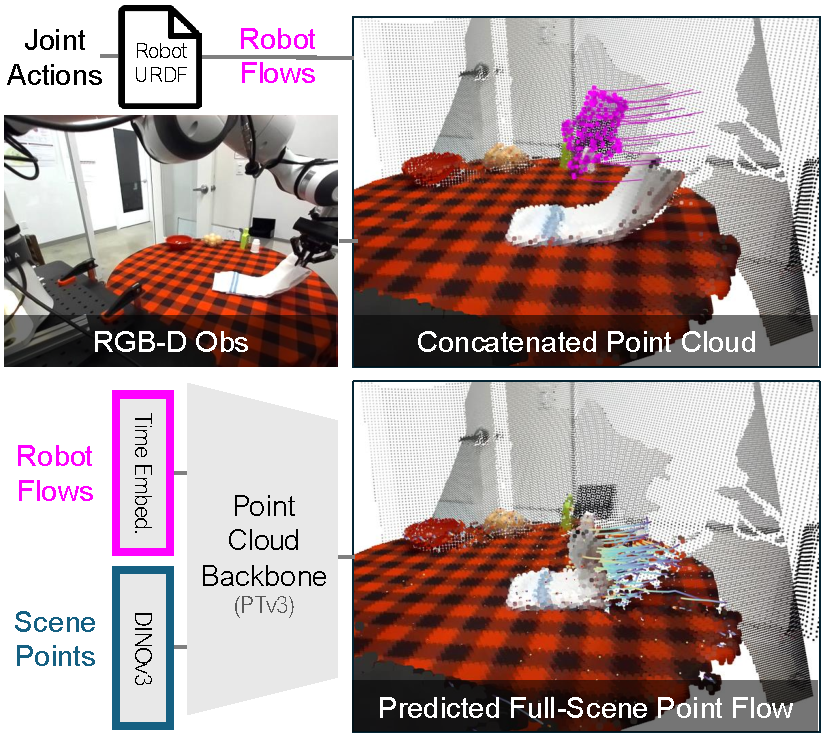
\includegraphics[height=#1]{figs/fig2_overview.pdf}};
    \begin{scope}[x={(arch.south east)},y={(arch.north west)}]
      \ifcase#2\relax
      \or % 1: RGB-D observation.
        \pwarchrect{0.004}{0.505}{0.414}{0.846}
      \or % 2: Full robot-action input.
        \pwarchrect{0.002}{0.851}{0.421}{0.997}
        \pwarchrect{0.002}{0.251}{0.220}{0.489}
      \or % 3: PTv3 backbone.
        \pwarchrect{0.224}{0.012}{0.414}{0.488}
      \or % 4: Concatenated point cloud.
        \pwarchrect{0.427}{0.502}{0.998}{0.978}
      \or % 5: Predicted full-scene point flow.
        \pwarchrect{0.427}{0.014}{0.998}{0.489}
      \or % 6: Scene points and DINOv3.
        \pwarchrect{0.002}{0.012}{0.219}{0.245}
      \or % 7: URDF and joint-action conversion.
        \pwarchrect{0.002}{0.851}{0.421}{0.997}
      \or % 8: Robot flows and time embedding.
        \pwarchrect{0.002}{0.251}{0.220}{0.489}
      \fi
    \end{scope}
    \pgfresetboundingbox
    \path[use as bounding box]
      (arch.south west) rectangle (arch.north east);
  \end{tikzpicture}%
}

\begin{frame}{Architecture overview}
  \centering
  \paperfig{height=5.7cm}{figs/fig2_overview.pdf}{Fig.~2}
\end{frame}


\begin{frame}{Architecture: scene state}
  \centering

  \begin{tikzpicture}
    \node[anchor=south west,inner sep=0pt] (arch) at (0,0)
      {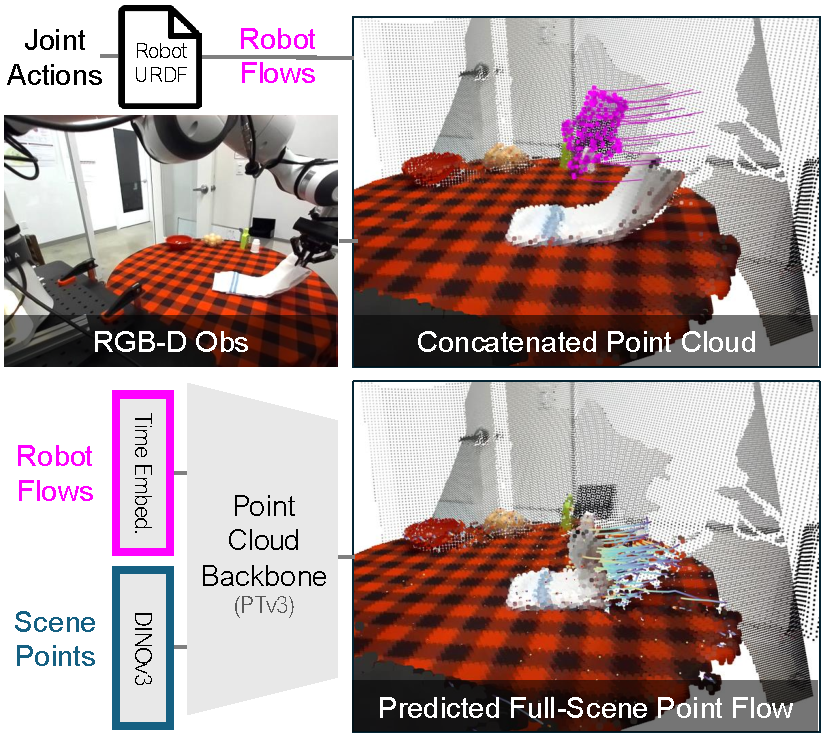
\includegraphics[height=5.7cm]{figs/fig2_overview.pdf}};

    \begin{scope}[x={(arch.south east)},y={(arch.north west)}]
      % Highlight RGB-D observation
      \pwarchrect{0.004}{0.505}{0.414}{0.846}

      % Highlight scene points + DINOv3 features
      \pwarchrect{0.002}{0.012}{0.219}{0.245}
    \end{scope}
  \end{tikzpicture}

  \credit{Fig.~2, highlighted; \S3.1}
\end{frame}

\begin{frame}[t]{Scene state representation: 3D points and visual features}
\vspace{-0.3cm}

{\centering\small
  $\displaystyle
    \mathbf s_t
    =\{(\mathbf p_{t,i},\mathbf f_i^S)\}_{i=1}^{N_S}
  $\par
}

\vspace{0.7cm}
\begin{columns}[t]
  \column{0.48\textwidth}
  \uncover<1->{
    {\small\bfseries\color{pw}3D positions:
      $\mathbf p_{t,i}\in\mathbb R^3$}\par
    \vspace{6pt}
    \footnotesize
    \begin{itemize}\setlength{\itemsep}{9pt}
      \item Back-project calibrated RGB-D into a 3D scene point cloud.
      \item $\mathbf p_{t,i}$ is point $i$'s position at time $t$;
        $N_S$ is the number of observed scene points.
    \end{itemize}
  }

  \column{0.48\textwidth}
  \uncover<2->{
    {\small\bfseries\color{pw}Visual features:
      $\mathbf f_i^S\in\mathbb R^{D_S}$}\par
    \vspace{6pt}
    \footnotesize
    \begin{itemize}\setlength{\itemsep}{9pt}
      \item Attach features from a \textbf{frozen DINOv3 encoder}
        at corresponding image locations.
      \item These features provide appearance and objectness cues.
      \item The feature vector stays fixed during the imagined rollout.
    \end{itemize}
  }
\end{columns}
\vfill
\credit{\S3.1; \S5.1, pretrained 2D features}
\end{frame}


\begin{frame}{Architecture: robot action}
  \centering

  \begin{tikzpicture}
    \node[anchor=south west,inner sep=0pt] (arch) at (0,0)
      {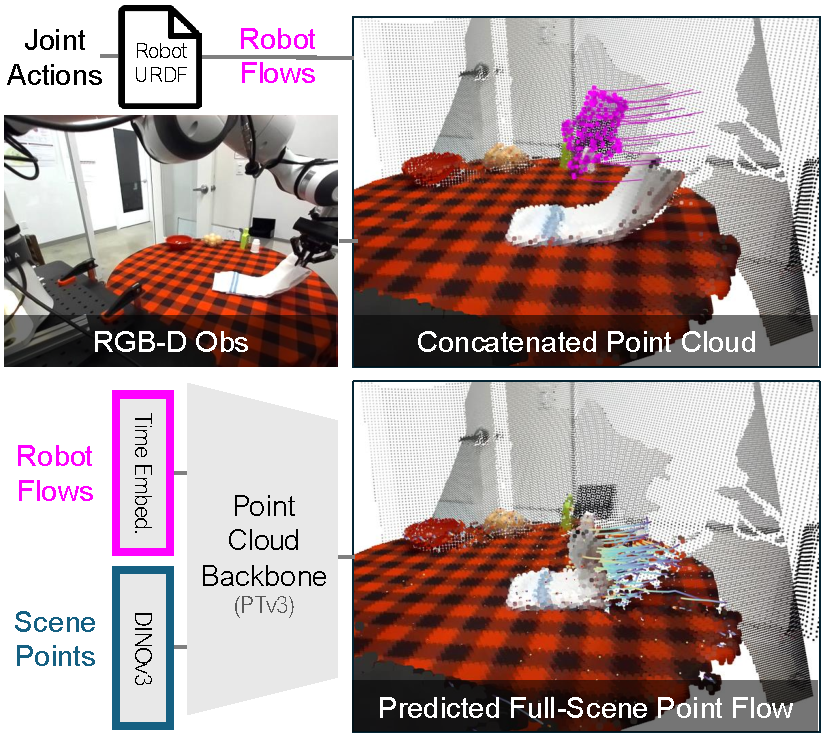
\includegraphics[height=5.7cm]{figs/fig2_overview.pdf}};

    \begin{scope}[x={(arch.south east)},y={(arch.north west)}]
      % Top: URDF and proposed robot joint trajectory
      \pwarchrect{0.002}{0.851}{0.421}{0.997}

      % Bottom: robot point flows and time embeddings
      \pwarchrect{0.002}{0.251}{0.220}{0.489}
    \end{scope}
  \end{tikzpicture}

  \credit{Fig.~2, highlighted; \S3.1}
\end{frame}




\begin{frame}{Robot action representation: joints to 3D points}
  \vspace{-5pt}
  \[
    \mathbf r_{t+k,j}
    =
    \operatorname{FK}_{\mathrm{URDF}}
    (\mathbf q_{t+k},\mathbf u_j)
  \]

  \begin{columns}[T,onlytextwidth]
    \column{0.49\textwidth}
    {\small\bfseries\color{pw}Given robot geometry and motion}\par
    \vspace{6pt}
    \footnotesize
    \begin{itemize}\setlength{\itemsep}{9pt}
      \item<1-> \textbf{URDF}: robot links, joints, and geometry.
      \item<2-> $\mathbf u_j$: a sampled surface point fixed to a robot link.
      \item<3-> $\mathbf q_{t+k}$: proposed joint configuration at future step $k$.
    \end{itemize}

    \column{0.47\textwidth}
    {\small\bfseries\color{pw}Construct the point-flow action}\par
    \vspace{6pt}
    \footnotesize
    \begin{itemize}\setlength{\itemsep}{10pt}
      \item<4-> Forward kinematics computes each point's future 3D position,
        $\mathbf r_{t+k,j}$.
      \item<4-> Repeat over the proposed trajectory.
        In practice, sample \pw{300--500 points per gripper}.
    \end{itemize}
  \end{columns}
  \vfill
  \credit{\S3.1, action representation; \S5.2}
\end{frame}


\begin{frame}{Architecture: predicting 3D displacement}
  \begin{columns}[c]

    \column{0.48\textwidth}
      \centering
      % Highlight follows the explanation.
      \only<1>{\pwarchitecturefocus{5.0cm}{4}}
      \only<2>{\pwarchitecturefocus{5.0cm}{3}}
      \only<3->{\pwarchitecturefocus{5.0cm}{5}}

    \column{0.48\textwidth}
      \footnotesize
      \begin{itemize}\setlength{\itemsep}{10pt}

        \item<1-> \textbf{Combine inputs}:
          concatenate scene points and proposed robot
          point trajectories into one point cloud.

        \item<2-> \textbf{PTv3 backbone}:
          process the combined cloud to produce
          learned features for each point.

        \item<3-> \textbf{MLP prediction head}:
          convert scene-point features into
          3D displacements.

      \end{itemize}

    
  \end{columns}
  \credit{Fig.~2, highlighted; \S3.1;
    PTv3 \citep{wu2023ptv3}}
\end{frame}


\begin{frame}[t]{Prediction horizon = 10 future states at once}
\vspace{-0.25cm}
\small

\textbf{Single-step prediction}
\[
  \hat{\mathbf s}_{t+1}
  =
  \mathcal F_\theta(\mathbf s_t,\mathbf a_t)
\]
{\footnotesize
  Predict one future state, then repeat to look further ahead.
\par}

\vspace{10pt}

\uncover<2->{
  \textbf{\pw{PointWorld: chunked prediction}}
  \[
    \mathcal F_\theta^H
    \big(\mathbf s_t,\mathbf a_{t:t+H-1}\big)
    =
    \hat{\mathbf s}_{t+1:t+H}
  \]
  {\footnotesize
    Predict $H=10$ future states in one forward pass:
    $0.1\,\mathrm{s}$ per step, covering $1\,\mathrm{s}$.
  \par}
}

\vspace{10pt}

\uncover<3->{
  {\footnotesize\bfseries Advantages}\par
  \begin{itemize}\setlength{\itemsep}{6pt}
    \item \footnotesize Better temporal consistency
      and less rollout drift.
    \item \footnotesize One forward pass per chunk,
      rather than repeated single-step predictions.
  \end{itemize}
}

\vfill
\credit{\S3.1; chunking ablation in \S5.2, Fig.~12}
\end{frame}


\begin{frame}{Training objective: Huber residual}
  \small
  \pwequation{1}
  \vspace{7pt}

  \begin{itemize}
    \footnotesize
    \setlength{\itemsep}{9pt}

    \item<1-> $\hat{\mathbf P}_{t+k,i}$ and $\mathbf P_{t+k,i}$: predicted and ground-truth future positions.

    \item<2-> Position error equals displacement error since the initial point is shared.

    \item<3-> $\rho_\delta$ is the elementwise \textbf{Huber loss}: quadratic for small residuals and linear for large ones, reducing sensitivity to noisy labels.

  \end{itemize}

  \vfill
  {\scriptsize\color{mute}
    Sum over future steps $k=1,\ldots,H$ and scene points $i=1,\ldots,N_S$.
  \par}
  \credit{Eq.~1, \S3.1}
\end{frame}


\begin{frame}{Training objective: emphasize moving points}
  \vspace{-12pt}\small\setlength{\abovedisplayskip}{5pt}\setlength{\belowdisplayskip}{5pt}
  \pwequation{2}
  \[
    m_{k,i}=\sigma\!\left(\kappa(\delta_{k,i}-\tau)\right),
    \qquad
    w_{k,i}=\frac{m_{k,i}}{\sum_{k,i}m_{k,i}}.
  \]
  \begin{itemize}\setlength{\itemsep}{7pt}
    \item<1-> \footnotesize Only about \pw{1--5\%} of scene points move. An unweighted loss is dominated by static background.
    \item<2-> $\delta_{k,i}$ is ground-truth displacement magnitude, $\tau$ a threshold, $\kappa$ the sigmoid sharpness, and $\sigma$ the logistic sigmoid.
    \item<3-> Normalize movement likelihoods into weights, giving moving points more training signal.
  \end{itemize}
  \credit{Eq.~1, \S3.1; \S5.1}
\end{frame}

\begin{frame}{Training objective: uncertainty weight}
  \small
  \pwequation{3}
  \centering
  \paperfig{width=0.76\linewidth,trim=0 0 0 129,clip}{figs/fig4_weighting.pdf}{Fig.~4, bottom row}
  \vspace{5pt}
  \begin{notes}[0.93\linewidth]
    \item<1-> The network predicts a scalar log-variance $s_{k,i}$ for each point and timestep, without uncertainty labels.
    \item<2-> Larger $s_{k,i}$ gives smaller $e^{-s_{k,i}}$, reducing the influence of unreliable residuals.
  \end{notes}
  \credit{Eq.~1, \S3.1}
\end{frame}


\begin{frame}{Training objective: uncertainty regularizer}
  \vspace{-12pt}
  \small
  \setlength{\abovedisplayskip}{5pt}
  \setlength{\belowdisplayskip}{5pt}

  \pwequation{4}
  \vspace{8pt}

  \footnotesize
  \begin{itemize}\setlength{\itemsep}{11pt}
    \item<1-> Without the $+s_{k,i}$ term, the model could suppress residual loss by making predicted uncertainty arbitrarily large.

    \item<2-> The regularizer penalizes that escape, balancing residual fit against predicted uncertainty.

    \item<3-> Together, Huber loss, movement weighting, and uncertainty regularization stabilize training on noisy real-world point flows.
  \end{itemize}

  \vfill
  {\scriptsize\color{mute}
    Points marked invisible by the annotation tracker are excluded from supervision.
  \par}
  \credit{Eq.~1, \S3.1; \S5.1}
\end{frame}


\begin{frame}{PointWorld for robotic manipulation}
  \centering
  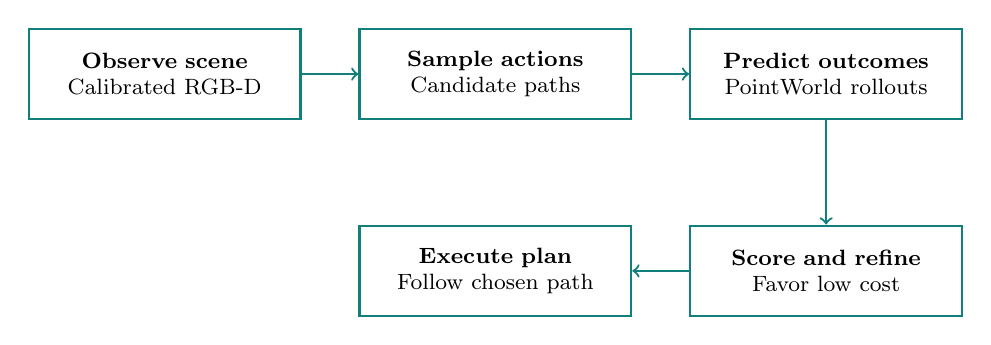
\begin{tikzpicture}[
    every node/.style={font=\footnotesize,align=center},
    stage/.style={draw=pw,thick,text width=3.1cm,minimum height=1.15cm,inner sep=5pt}
  ]
    \node[stage] (obs) at (0,1.5) {\textbf{Observe scene}\\Calibrated RGB-D};
    \uncover<2->{
      \node[stage] (sample) at (4.2,1.5) {\textbf{Sample actions}\\Candidate paths};
      \draw[->,thick,pw] (obs.east)--(sample.west);
    }
    \uncover<3->{
      \node[stage] (pred) at (8.4,1.5) {\textbf{Predict outcomes}\\PointWorld rollouts};
      \draw[->,thick,pw] (sample.east)--(pred.west);
    }
    \uncover<4->{
      \node[stage] (score) at (8.4,-1.0) {\textbf{Score and refine}\\Favor low cost};
      \draw[->,thick,pw] (pred.south)--(score.north);
    }
    \uncover<5->{
      \node[stage] (act) at (4.2,-1.0) {\textbf{Execute plan}\\Follow chosen path};
      \draw[->,thick,pw] (score.west)--(act.east);
    }
  \end{tikzpicture}
  \vfill
 
  \vspace{5pt}
  \credit{\S3.2; real-robot appendix}
\end{frame}


\begin{frame}{MPPI: sampling and optimizing robot trajectories}

  \begin{columns}[c]

    % LEFT: Trajectory visualization
    \column{0.43\textwidth}
      \centering
      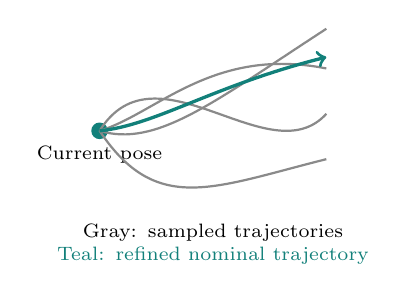
\begin{tikzpicture}[x=0.72cm,y=0.72cm]

        \fill[pw] (0,0) circle (3pt);
        \node[font=\scriptsize,anchor=north]
          at (0,-0.1) {Current pose};

        % Candidate trajectories
        \uncover<1->{
          \draw[mute,thick]
            (0,0)..controls(1,0.3)and(2,1.5)..(4,1.1);
          \draw[mute,thick]
            (0,0)..controls(1,1.6)and(3,-0.8)..(4,0.3);
          \draw[mute,thick]
            (0,0)..controls(1,-1.5)and(2,-1)..(4,-0.5);
          \draw[mute,thick]
            (0,0)..controls(1,-0.3)and(2,0.5)..(4,1.8);
        }

        % Refined nominal trajectory
        \uncover<3->{
          \draw[pw,very thick,->]
            (0,0)..controls(1,0.1)and(2,0.8)..(4,1.3);
        }

        \node[font=\scriptsize,text width=4cm,
              align=center]
          at (2,-2) {
            Gray: sampled trajectories\\
            \textcolor{pw}{Teal: refined nominal trajectory}
          };

      \end{tikzpicture}

    % RIGHT: Technical steps
    \column{0.55\textwidth}

      \footnotesize
      \begin{itemize}
        \setlength{\itemsep}{11pt}

        \item<1-> \textbf{Sample trajectories:}
          Generate $K$ candidate end-effector
          trajectories using time-correlated
          cubic-spline perturbations.

        \item<2-> \textbf{Predict and evaluate:}
          Convert each candidate into robot
          point flows; use PointWorld to predict
          scene motion and compute cost $J^{(\ell)}$.

        \item<3-> \textbf{Update nominal trajectory:}
          Weight candidates by their costs:
      \end{itemize}

      \uncover<3->{
        \vspace{-5pt}
        \[
          \omega_\ell =
          \frac{\exp(-J^{(\ell)}/\beta)}
               {\sum_{\ell'}\exp(-J^{(\ell')}/\beta)}
        \]
      }

  \end{columns}

  \vfill


  \credit{\S3.2; MPPI \citep{williams2017mppi}}
\end{frame}



\begin{frame}{Planning cost: task success + robot motion}

  \vspace{-8pt}
  \small
  \[
    \underset{\mathbf E_{0:T}}{\operatorname{arg\,min}}
    \sum_{k=1}^{T}
    \left[
      \underbrace{c_{\mathrm{task}}(\mathbf s_k)}_{\text{Task cost}}
      +
      \underbrace{c_{\mathrm{ctrl}}(\mathbf E_k)}_{\text{Control cost}}
    \right]
  \]

  \vspace{6pt}

  \begin{itemize}
    \footnotesize
    \setlength{\itemsep}{15pt}

    \item<1-> \textbf{Task cost:} How close does the
      predicted scene get to the desired target?
      \vspace{-4pt}
      \[
        c_{\mathrm{task}}(\mathbf s_k)
        =
        \frac{1}{|\mathcal I_{\mathrm{task}}|}
        \sum_{i\in\mathcal I_{\mathrm{task}}}
        \|\mathbf p_{k,i}-\mathbf g_i\|_2^2
      \]
      {\scriptsize
        $\mathbf p_{k,i}$: predicted point position;
        $\mathbf g_i$: target position;
        $\mathcal I_{\mathrm{task}}$: selected points.
      \par}

    \item<2-> \textbf{Control cost:}
      Evaluates the end-effector trajectory
      $\mathbf E_{0:T}$ by penalizing:
      \begin{itemize}
        \item Excessive travel distance between poses.
        \item Unreachable end-effector poses.
      \end{itemize}

  \end{itemize}

  \vfill


  \credit{Eq.~2, \S3.2}
\end{frame}


%% ==== HANDOFF ====

%% ---- Part B (Juntang, S4-6) ----
% Layout: figure centred, bullets from the left margin, footer pinned to the bottom
% (backup links left, source right). No credits under figures in this half.

% Figure; #3 draws on it in coordinates normalized to the figure.
\newcommand{\pwfig}[3]{%
  \begin{tikzpicture}[baseline=(f.south)]
    \node[anchor=south west, inner sep=0pt] (f) at (0,0) {\includegraphics[#1]{#2}};
    \begin{scope}[x={(f.south east)}, y={(f.north west)}] #3 \end{scope}
  \end{tikzpicture}}
% Footer: #1 bottom-left (backup links), #2 bottom-right (source), on one baseline.
\newcommand{\foot}[2]{\par\nointerlineskip\noindent\begin{tikzpicture}[remember picture, overlay]
  \node[anchor=base west, inner sep=0pt, font=\tiny, text=mute]
    at ([shift={(0.55cm,0.32cm)}]current page.south west) {#1};
  \node[anchor=base east, inner sep=0pt, font=\tiny, text=mute]
    at ([shift={(-1.15cm,0.32cm)}]current page.south east) {#2};\end{tikzpicture}}
\newcommand{\pwsrc}[1]{\citet{huang2026pointworld}, #1}
\newcommand{\bk}[2]{\hyperlink{#1}{\color{cite}#2}}
% Extra detail in small gray type, aligned with the bullets.
\newcommand{\aside}[1]{{\par\raggedright\tiny\color{mute}#1\par}}
% Model name after a step, small and gray; citations live in the pipeline backup.
\newcommand{\tool}[1]{ {\scriptsize\color{mute}(#1)}}
% Box a table cell on one overlay without moving the table.
\newcommand{\cellbox}[2]{\alt<#1>{\tikz[baseline=(n.base)]{\node[inner sep=0pt] (n) {#2};
  \draw[overlay, orange!90!red, line width=1.6pt, rounded corners=1pt]
    ([shift={(-3pt,-3pt)}]n.south west) rectangle ([shift={(3pt,3pt)}]n.north east);}}{#2}}

% Data 1:15. S4, Fig. 5
\begin{frame}[label=data]{Data: re-annotating DROID in 3D}
  \centering
  \pwfig{height=4.3cm}{figs/fig5a_annotation.pdf}{%
    \only<1>{\pwarchrect{0.668}{0.005}{0.997}{1.06}}%
    \only<2>{\pwarchrect{0.335}{0.005}{0.664}{1.06}}}
  \vfill
  \begin{notes}[\linewidth]
    \item<1-> \textbf{Original}: DROID's depth and camera poses are noisy.
    \item<2-> \textbf{Ours}: depth\tool{FoundationStereo}, cameras\tool{VGGT + robot
      mesh}, 3D tracks\tool{CoTracker3}.
    \item<3-> \textbf{Scale}: \pw{about 2M trajectories, 500 hours}, real and simulated.
  \end{notes}
  \vfill
  \foot{Backup: \bk{bk-pipeline}{pipeline} $\cdot$ \bk{bk-quality}{quality} $\cdot$
      \bk{bk-b1k}{BEHAVIOR-1K}}
    {\pwsrc{Fig.~5} $\cdot$ DROID \citep{khazatsky2024droid} $\cdot$ BEHAVIOR-1K
      \citep{li2024behavior}}
\end{frame}

% Evaluation 0:45. S4, Fig. 6
\begin{frame}[label=eval]{Evaluation: how predictions are scored}
  \centering
  \pwfig{width=0.92\linewidth, trim=16 485 0 0, clip}{figs/fig6_rollouts.pdf}{%
    \only<1>{\pwarchrect{0.396}{0.01}{0.997}{1.08}}}
  \vfill
  \begin{notes}[\linewidth]
    \item<1-> \textbf{$\ell_2$ mover}: average 3D error of the points that move.
    \item<2-> \textbf{Filtering}: on real data, only points an expert model trusts count.
    \item<3-> \textbf{Units}: \pw{metres, so 0.001 is 1\,mm.}
  \end{notes}
  \vfill
  \foot{Backup: \bk{bk-eval}{evaluation details}}{\pwsrc{Fig.~6, \S4}}
\end{frame}

% Roadmap 1:00. Fig. 7, S5.1
\begin{frame}[label=roadmap]{Roadmap: what each change bought}
  \begin{columns}[c]
    \column{0.40\textwidth}
      \centering
      \pwfig{height=5.9cm}{figs/fig7_roadmap.pdf}{%
        \only<1>{\pwarchrect{-0.03}{0.756}{1.06}{0.962}}%
        \only<2>{\pwarchrect{-0.03}{0.290}{1.06}{0.758}}%
        \only<3>{\pwarchrect{-0.03}{0.091}{1.06}{0.292}}%
        \only<4>{\pwarchrect{0.20}{0.893}{1.06}{0.962}\pwarchrect{0.20}{0.091}{1.06}{0.152}}}
    \column{0.56\textwidth}
      \footnotesize
      \begin{itemize}\setlength{\itemsep}{10pt}
        \item<1-> \textbf{Backbone}: PTv3, the biggest gain, 3.8\,mm.
        \item<2-> \textbf{Loss and DINO features}: 1.7\,mm.
        \item<3-> \textbf{Model size}, 50M $\to$ 1B: 1.9\,mm.
        \item<4-> \textbf{Total}: \pw{7.4\,mm, 19\% less error.}
      \end{itemize}
  \end{columns}
  \foot{Backup: \bk{bk-backbones}{all backbones}}{\pwsrc{Fig.~7, \S5.1}}
\end{frame}

% Scaling 0:45. Fig. 9, S5.2, Tab. 1
\begin{frame}[label=scaling]{Scaling: data and model size}
  \begin{columns}[c]
    \column{0.40\textwidth}
      \centering
      \pwfig{height=4.6cm}{figs/fig9_scaling.pdf}{%
        \only<1>{\fill[white, opacity=0.75] (0.597,0) rectangle (1,1);}%
        \only<2-3>{\fill[white, opacity=0.75] (0.17,0) rectangle (0.594,1);}}
    \column{0.56\textwidth}
      \footnotesize
      \begin{itemize}\setlength{\itemsep}{10pt}
        \item<1-> \textbf{Data}: error falls log-linearly with data.
        \item<2-> \textbf{Model}: same trend, up to 1B parameters.
        \item<3-> \textbf{Speed}: 0.12\,s per prediction at 1B.
        \item<4-> \pw{Predictable gains from scale.}
      \end{itemize}
  \end{columns}
  \foot{Backup: \bk{bk-backbones}{all backbones}}{\pwsrc{Fig.~9, Tab.~1, \S5.2}}
\end{frame}

% Generalization 1:00. Tab. 2 held-out columns, S5.3
\begin{frame}[label=transfer]{Generalization: transfer to a new lab}
  \vfill
  {\centering\small
  \setlength{\tabcolsep}{9pt}
  \begin{tabular}{@{}lcccc@{}}
    \toprule
    pretrained on & DROID & BEHAVIOR-1K & \pw{both} & \cellbox{1}{specialist (H only)} \\
    \midrule
    zero-shot & 0.0305 & 0.0531 & \cellbox{2}{\pw{0.0300}} & \cellbox{2}{0.0293} \\
    finetuned & \textbf{0.0271} & 0.0299 & \cellbox{3}{\pw{\textbf{0.0272}}} & \cellbox{3}{0.0293} \\
    \bottomrule
  \end{tabular}\par
  \vspace{3pt}{\tiny\color{mute} $\ell_2$ mover on the held-out lab H; lower is better.}\par}
  \vfill
  \begin{notes}[\linewidth]
    \item<1-> \textbf{Setup}: lab H is held out; a specialist trains on H only.
    \item<2-> \textbf{Zero-shot}: within 0.7\,mm of the specialist.
    \item<3-> \textbf{Finetuned}: \pw{beats it by 2.1\,mm, with 20$\times$ fewer steps.}
  \end{notes}
  \vfill
  \foot{Backup: \bk{bk-transfer}{all transfer results}}{\pwsrc{Tab.~2, \S5.3}}
\end{frame}

% Real robot 1:15. Fig. 8, S5.4, App. A.6
\begin{frame}[label=robot]{Real robot: zero-shot planning}
  \centering
  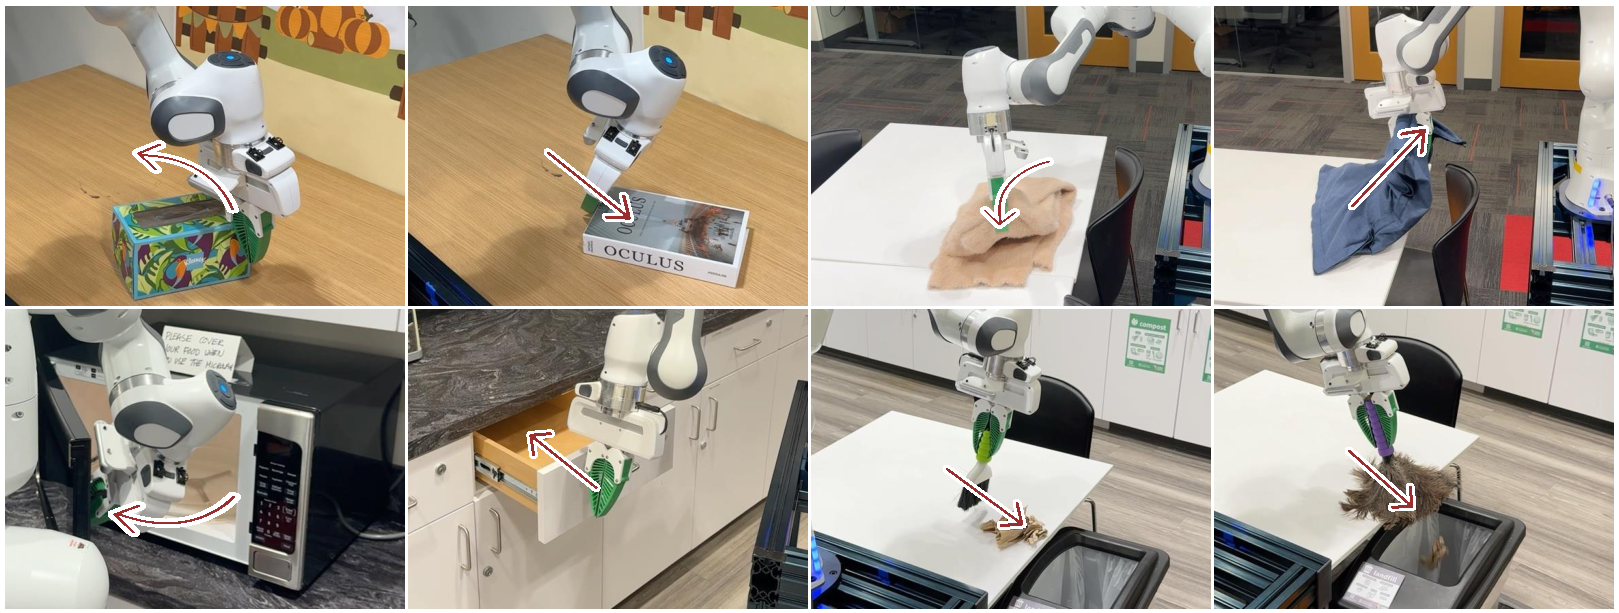
\includegraphics[height=2.7cm]{figs/fig8b_tasks.pdf}\\[2pt]
  \uncover<2->{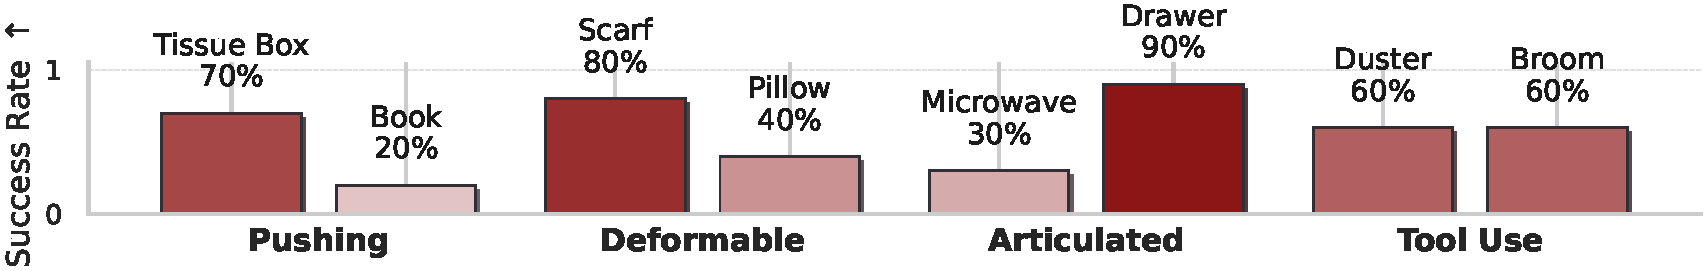
\includegraphics[width=0.86\linewidth]{figs/fig8a_success.pdf}}
  \vfill
  \begin{notes}[\linewidth]
    \item<1-> \textbf{Setup}: 8 tasks, 10 trials each, an unseen gripper, no demos.
    \item<2-> \textbf{Result}: \pw{45 of 80 trials succeed (56\%).}
      Videos: \href{https://point-world.github.io}{point-world.github.io}
  \end{notes}
  \vfill
  \foot{Backup: \bk{bk-protocol}{robot protocol} $\cdot$ \bk{bk-ablations}{horizon and
      cameras}}{\pwsrc{Fig.~8, \S5.4, App.~A.6}}
\end{frame}

% Limitations 0:30. App. A.1
\begin{frame}[label=limits]{Limitations}
  \vfill
  \small
  \begin{itemize}\setlength{\itemsep}{16pt}
    \item<1-> \textbf{Static input}: the scene must start at rest.
    \item<2-> \textbf{Manual goals}: masks and targets are set by hand.
    \item<3-> \textbf{Ideal robot}: rigid, and follows its plan exactly.
  \end{itemize}
  \vfill
  \foot{Backup: \bk{bk-reading}{our reading}}{\pwsrc{App.~A.1}}
\end{frame}

% Takeaway 0:30
\begin{frame}{Takeaway}
  \vfill
  \small
  \begin{itemize}\setlength{\itemsep}{16pt}
    \item<1-> One \pw{3D world model}: scene and robot as moving points.
    \item<2-> \pw{Scale keeps helping}: more data, bigger models.
    \item<3-> \pw{Zero-shot planning} on a real robot, from one image.
  \end{itemize}
  \vfill
\end{frame}

% Discussion: the 15 minutes end here; hand over to the roles in the agreed order.
\begin{frame}[label=discussion]{Discussion}
  \vfill
  \small
  \begin{itemize}\setlength{\itemsep}{16pt}
    \item<1-> \textbf{Planning}: no baseline, no replanning. Is 56\% good?
    \item<2-> \textbf{Action}: on real data, a plain gripper pose comes close. Why points?
    \item<3-> \textbf{Scope}: one still frame, about 3\,cm error. What is out of reach?
  \end{itemize}
  \vfill
  \foot{Backup: \bk{bk-action}{why gripper points} $\cdot$ \bk{bk-reading}{our reading}}{}
\end{frame}

%% ---- backup: same order as the main slides; each links back ----
\appendix

% App. A.2 (A.2.2 cameras, A.2.4 tracks); S4
\begin{frame}[label=bk-pipeline]{Backup: DROID annotation pipeline}
  \centering
  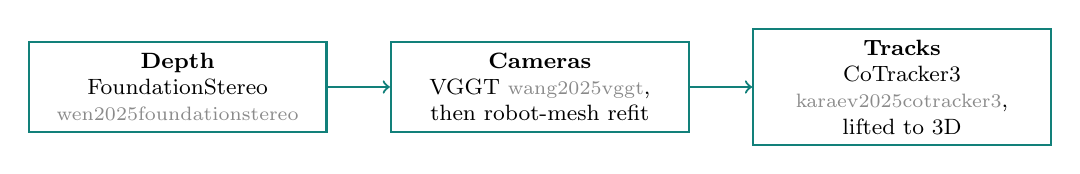
\begin{tikzpicture}[
    every node/.style={font=\footnotesize, align=center},
    stage/.style={draw=pw, thick, text width=3.5cm, minimum height=1.0cm, inner sep=4pt}]
    \node[stage] (d) at (0,0) {\textbf{Depth}\\FoundationStereo \src{wen2025foundationstereo}};
    \node[stage] (c) at (4.6,0) {\textbf{Cameras}\\VGGT \src{wang2025vggt}, then robot-mesh refit};
    \node[stage] (t) at (9.2,0) {\textbf{Tracks}\\CoTracker3 \src{karaev2025cotracker3}, lifted to 3D};
    \draw[->, thick, pw] (d) -- (c);
    \draw[->, thick, pw] (c) -- (t);
  \end{tikzpicture}
  \vfill
  \begin{notes}[\linewidth]
    \item \textbf{Initialize}: VGGT poses the cameras; the wrist camera ties them to the robot.
    \item \textbf{Render}: the robot mesh at the recorded joint angles, seen from each camera.
    \item \textbf{Match}: refit all cameras jointly to minimize robot depth error,
      $\frac1K\sum |d^{\text{obs}} - d^{\text{pred}}|$.
    \item \textbf{Result}: \pw{reliable camera poses for about 60\% of DROID episodes.}
  \end{notes}
  \vspace{8pt}
  \aside{VGGT alone can be off by tens of cm. Tracks run on non-robot workspace pixels;
    occluded points get no loss.}
  \vfill
  \foot{$\leftarrow$ Back to \bk{data<3>}{Data}}{\pwsrc{App.~A.2}}
\end{frame}

% Fig. 5 bottom, App. A.2.3
\begin{frame}[label=bk-quality]{Backup: annotation quality}
  \centering
  \pwfig{width=0.92\linewidth}{figs/fig5b_cdf.pdf}{}
  \vfill
  \begin{notes}[\linewidth]
    \item \textbf{Left}: depth error on the robot's own surface.
    \item \textbf{Middle, right}: two cameras' point clouds agree within 5 and 20\,mm.
    \item \textbf{Result}: \pw{higher curves are better; ours is on top almost everywhere.}
    \item \textbf{Cameras}: a median 1.8\,cm and 1.9$^\circ$ from a proxy truth.
  \end{notes}
  \vspace{8pt}
  \aside{Proxy truth: the best 1\% of scenes under DROID's own calibration.}
  \vfill
  \foot{$\leftarrow$ Back to \bk{data<3>}{Data}}{\pwsrc{Fig.~5, \S4, App.~A.2.3}}
\end{frame}

% S4 "Simulation"; App. A.3; Fig. 19; Tab. 2
\begin{frame}[label=bk-b1k]{Backup: BEHAVIOR-1K simulation data}
  \centering
  \pwfig{width=0.52\linewidth, trim=0 474 0 0, clip}{figs/fig19_b1k_rollouts.pdf}{}
  \vfill
  \begin{notes}[\linewidth]
    \item \textbf{Source}: BEHAVIOR-1K \src{li2024behavior}, 10k episodes, 50 household tasks.
    \item \textbf{Robot}: Galaxea R1 Pro, two arms on a mobile base.
    \item \textbf{Labels}: exact flows, read from the simulator state.
    \item \textbf{Role}: \pw{alone, weak on real data (0.0531); with DROID, the best mix (0.0300).}
  \end{notes}
  \vspace{8pt}
  \aside{1,100\,h of teleoperation before filtering, replayed in Isaac Sim with three
    robot-mounted cameras. Role: zero-shot $\ell_2$ mover, held-out lab.}
  \vfill
  \foot{$\leftarrow$ Back to \bk{data<3>}{Data}}{\pwsrc{Fig.~19, App.~A.3, Tab.~2}}
\end{frame}

% S4 evaluation protocol; App. A.5
\begin{frame}[label=bk-eval]{Backup: evaluation details}
  \vfill
  \footnotesize
  \begin{itemize}\setlength{\itemsep}{14pt}
    \item \textbf{Metric}: $\ell_2$ per point and per step over 1\,s, averaged per sequence.
    \item \textbf{Movers}: set by the true motion; static points are scored on their own.
    \item \textbf{Expert filter}: trained only on the test split; keeps the 80\% it trusts
      most (\S4).
    \item \textbf{Same for all}: \pw{every model is scored on the same filtered test set.}
  \end{itemize}
  \vspace{10pt}
  \aside{BEHAVIOR-1K labels are noiseless and not filtered. The authors: this dense metric
    exposes differences that task success rates miss.}
  \vfill
  \foot{$\leftarrow$ Back to \bk{eval<3>}{Evaluation}}{\pwsrc{\S4, App.~A.5}}
\end{frame}

% Tab. 1
\begin{frame}[label=bk-backbones]{Backup: all backbones}
  \vfill
  {\centering\small
  \setlength{\tabcolsep}{5pt}
  \begin{tabular}{@{}lrrrrrr@{}}
    \toprule
    & params & memory & FLOPs & latency (ms) & $\ell_2$ mover & $\ell_2$ static \\
    \midrule
    GBND \src{ai2025review} & 1.00$\times$ & 1.00$\times$ & 1.00$\times$ & 13.46 & 0.0390 & 0.0066 \\
    PointNet & 1.03$\times$ & 0.34$\times$ & 0.04$\times$ & 5.93 & 0.0369 & 0.0084 \\
    PointNet++ & 1.07$\times$ & 0.67$\times$ & 0.06$\times$ & 327.08 & 0.0368 & 0.0073 \\
    SparseConv & 33.31$\times$ & 7.18$\times$ & 1.32$\times$ & 17.70 & 0.0396 & 0.0076 \\
    Transformer & 41.06$\times$ & 0.31$\times$ & 3.38$\times$ & 30.43 & 0.0339 & 0.0071 \\
    \pw{PTv3-50M} & 49.14$\times$ & 0.30$\times$ & 0.34$\times$ & 59.60 & 0.0331 & 0.0067 \\
    \pw{PTv3-132M} & 127.22$\times$ & 0.69$\times$ & 1.04$\times$ & 69.60 & 0.0324 & 0.0061 \\
    \pw{PTv3-411M} & 398.67$\times$ & 1.89$\times$ & 1.90$\times$ & 102.47 & 0.0315 & 0.0059 \\
    \pw{PTv3-1B} & 957.71$\times$ & 4.30$\times$ & 3.57$\times$ & 123.65 & \textbf{0.0312}
      & \textbf{0.0056} \\
    \bottomrule
  \end{tabular}\par
  \vspace{3pt}{\tiny\color{mute} Params, memory and FLOPs relative to GBND.}\par}
  \vfill
  \begin{notes}[\linewidth]
    \item \textbf{GBND}: a feature per point and local messages; memory grows fast, far
      effects get lost.
  \end{notes}
  \vfill
  \foot{$\leftarrow$ Back to \bk{roadmap<4>}{Roadmap} $\cdot$ \bk{scaling<4>}{Scaling}}
    {\pwsrc{Tab.~1}}
\end{frame}

% Tab. 2, Fig. 10, S5.3
\begin{frame}[label=bk-transfer]{Backup: all transfer results}
  \centering
  {\scriptsize
  \setlength{\tabcolsep}{5pt}
  \begin{tabular}{@{}ll*{7}{c}c@{}}
    \toprule
    & & D$\to$D & B$\to$B & D$\to$B & B$\to$D & D$\to$H & B$\to$H & D+B$\to$H & specialist \\
    \midrule
    zero-shot & mover & 0.0315 & 0.0087 & 0.1460 & 0.0558 & 0.0305 & 0.0531 & 0.0300 & 0.0293 \\
      & static & 0.0059 & 0.0010 & 0.0050 & 0.0058 & 0.0049 & 0.0057 & 0.0063 & 0.0043 \\
    \midrule
    finetuned & mover & -- & -- & 0.0107 & 0.0378 & 0.0271 & 0.0299 & 0.0272 & 0.0293 \\
      & static & -- & -- & 0.0003 & 0.0086 & 0.0040 & 0.0046 & 0.0040 & 0.0043 \\
    \bottomrule
  \end{tabular}\par}
  \vspace{3pt}{\tiny\color{mute} D = DROID, B = BEHAVIOR-1K, H = held-out lab; pretrained
    $\to$ tested.}\par
  \vfill
  \pwfig{height=3.0cm}{figs/fig10_heldout.pdf}{}
  \vfill
  \aside{H is the CLVR lab within DROID, split 90/10; finetuned models see only the 90\%.
    Zero-shot between sim and real fails both ways (0.1460, 0.0558).}
  \vfill
  \foot{$\leftarrow$ Back to \bk{transfer<3>}{Generalization}}{\pwsrc{Tab.~2, Fig.~10}}
\end{frame}

% App. A.6
\begin{frame}[label=bk-protocol]{Backup: robot protocol}
  \vfill
  \small
  \begin{columns}[t, onlytextwidth]
    \column{0.48\textwidth}
      {\bfseries\color{pw} Planner}
      \begin{itemize}\setlength{\itemsep}{10pt}
        \item MPPI: 256 samples, 20 iterations.
        \item Spline noise, $\sigma$ from 0.05 to 0.50.
        \item 30 steps (3\,s) in 3 chunks, open loop.
      \end{itemize}
    \column{0.48\textwidth}
      {\bfseries\color{pw} Robot}
      \begin{itemize}\setlength{\itemsep}{10pt}
        \item Franka, unseen fin-ray gripper.
        \item One RealSense D435 camera.
        \item SAM~2 masks, GUI targets.
      \end{itemize}
  \end{columns}
  \vspace{14pt}
  \aside{MPPI temperature 0.05, EMA 0.9, cubic splines with 4 knots. Depth from the camera's
    IR stereo pair via FoundationStereo; masks from SAM~2 \citep{ravi2024sam2}. Training saw
    Robotiq and Galaxea R1 Pro grippers. Failures include plans judged unsafe to run.}
  \vfill
  \foot{$\leftarrow$ Back to \bk{robot<2>}{Real robot}}{\pwsrc{App.~A.6}}
\end{frame}

% Fig. 12 and Fig. 13, S5.2
\begin{frame}[label=bk-ablations]{Backup: horizon and cameras}
  \begin{columns}[t, onlytextwidth]
    \column{0.48\textwidth}
      {\small\bfseries\color{pw} Predict 1\,s at once}\par\vspace{6pt}
      {\centering\pwfig{height=3.3cm}{figs/fig12_chunk.pdf}{}\par}\vspace{8pt}
      \footnotesize
      \begin{itemize}\setlength{\itemsep}{4pt}
        \item \textbf{Chunked}: \pw{least drift}, in one pass.
        \item \textbf{Step by step}: drifts the most.
      \end{itemize}
    \column{0.48\textwidth}
      {\small\bfseries\color{pw} Number of cameras}\par\vspace{6pt}
      {\centering\pwfig{height=3.3cm}{figs/fig13_cameras.pdf}{}\par}\vspace{8pt}
      \footnotesize
      \begin{itemize}\setlength{\itemsep}{4pt}
        \item \textbf{More cameras} in training always help.
        \item \textbf{Random 1--3}: \pw{the most robust}.
      \end{itemize}
  \end{columns}
  \foot{$\leftarrow$ Back to \bk{robot<2>}{Real robot}}{\pwsrc{Figs.~12--13, \S5.2}}
\end{frame}

% Fig. 11, S5.2
\begin{frame}[label=bk-action]{Backup: why gripper points?}
  \begin{columns}[c, onlytextwidth]
    \column{0.40\textwidth}
      \centering
      \pwfig{height=4.15cm}{figs/fig11_action.pdf}{}
    \column{0.56\textwidth}
      \footnotesize
      \begin{itemize}\setlength{\itemsep}{10pt}
        \item \textbf{Compared}: gripper, whole body, pose, joints.
        \item \textbf{Result}: \pw{gripper points are best.}
        \item \textbf{Whole body}: loses to a pose on real data.
      \end{itemize}
      \vspace{8pt}
      \aside{Best on both real and simulated data; all trained on DROID and BEHAVIOR-1K. The
        authors' plausible explanation: many robot points obscure the sparse signal in noisy
        real data.}
  \end{columns}
  \foot{$\leftarrow$ Back to \bk{discussion<3>}{Discussion}}{\pwsrc{Fig.~11, \S5.2}}
\end{frame}

% Our critique for the reviewer and red-team roles. S4, S5, App. A.5-A.6
\begin{frame}[label=bk-reading]{Backup: our reading}
  \vfill
  \footnotesize
  \begin{itemize}\setlength{\itemsep}{9pt}
    \item \textbf{Robot}: 80 trials, no baseline, no replanning.
    \item \textbf{Setup}: deformable and tool tasks start with the object in hand.
    \item \textbf{Metric}: mm-level gaps, scored only where an expert model trusts the labels.
    \item \textbf{Filter}: \S4 keeps the top 80\%; the appendix's 0.8 quantile reads as top 20\%.
    \item \textbf{Transfer}: zero-shot is 0.7\,mm behind the specialist; clear wins need
      finetuning.
  \end{itemize}
  \vspace{10pt}
  \aside{Also: Fig.~11's legend says 3000 whole-body points where \S5.2 says 2000.}
  \vfill
  \foot{$\leftarrow$ Back to \bk{limits<3>}{Limitations} $\cdot$
    \bk{discussion<3>}{Discussion}}{\pwsrc{\S4, \S5, App.~A.5--A.6}}
\end{frame}

% No allowframebreaks: multicols would add a blank page.
\begin{frame}[t]{References}
  \vspace{-1.2em}
  \nocite{huang2026pointworld}
  {\tiny\linespread{0.84}\selectfont
  \setlength{\bibsep}{0.2pt plus 0.2pt}
  \setlength{\columnsep}{1em}
  \begin{multicols}{2}\bibliography{refs}\end{multicols}}
\end{frame}

\end{document}
